\documentclass[11pt,a4paper]{article}

\usepackage{amsmath,amssymb}
\usepackage{graphicx}
\usepackage{booktabs}
\usepackage{natbib}
\usepackage[margin=1in]{geometry}
\usepackage{enumitem}
\usepackage{hyperref}
\usepackage{xcolor}

\hypersetup{
  colorlinks=true,
  linkcolor=blue!50!black,
  citecolor=blue!50!black,
  urlcolor=blue!60!black
}

\graphicspath{{figures/}}

\title{GR Chapter 2: Off-center LTB sketch for Migkas anisotropy}
\author{C.\ A.}
\date{2026-09-20}

\begin{document}
\maketitle

\begin{abstract}
This note is a first-shot general-relativistic (GR) companion to the Newtonian
Sedov--Taylor + Center-of-Expansion (ST+CoE) synthesis. The backbone is
off-center dust Lema\^itre--Tolman--Bondi (LTB) geometry---optionally with
$\Lambda$---chosen as the simplest metric promotion of the Newtonian Gauss
enclosed-mass picture with radially decreasing density. We state the LTB
metric, encode a centrally concentrated toy $M(r)$, place an off-center
observer, and map a direction-dependent expansion rate to the Migkas
et~al.\ (2020) sheet convention $A\propto H_{\mathrm{obs}}/H$. A numerical
toy (FLRW-shell $H(r)$, not full null geodesics) yields affine
$R^2\approx0.43$ against digitised Migkas $A(\ell)$ after a sky-axis phase;
Amp$\times\sin$ and $2\ell$ remain diagnostic residuals, not free GR
parameters. The same toy, with a linear Hubble-gradient CMB dipole estimate,
places a horizon-scale offset ($d\sim0.5\,D$ with $D\sim c/H_0$) many orders
of magnitude above the observed CMB dipole, consistent with the
Alnes--Kodama $\sim15\,\mathrm{Mpc}$ ceiling class for spherical off-center
models. This is not a finished GR cosmology; it is an honest promotion of the
Newtonian sky template into metric language and an explicit CMB kill-shot
ledger.
\end{abstract}

\tableofcontents
\newpage

%----------------------------------------------------------------------
\section{Purpose}
\label{sec:purpose}

Chapter~1 of this program~\citep{Migkas2020} (Newtonian synthesis, companion
paper in this workspace) produced a phenomenological sky template: Sedov--Taylor
homology about a real Center of Expansion (CoE), off-center observer, Gauss
gravity from decreasing $\rho(r)$ (not a uniform ball $g\propto -r$), and a
sheet map
\begin{equation}
  A\;\propto\; H_{\mathrm{obs}}/H
  \label{eq:sheetAF}
\end{equation}
aimed at Migkas et~al.\ Fig.~6 $A$ versus Galactic longitude. Geometry alone
reached $R^2\approx0.543$; Amp$\times\sin$ (Amp$=-0.06$, $\phi\approx0.20\,\mathrm{rad}$)
raised $R^2\approx0.746$; a multiplicative $2\ell$ layer reached
$R^2\approx0.875$. Those last two layers are diagnostic, not first principles.

\paragraph{What this Chapter~2 does.}
\begin{enumerate}[leftmargin=*,itemsep=2pt]
\item Promote the Newtonian ST+Gauss sky template to a \textbf{metric}: dust
  LTB (optional $\Lambda$), with decreasing $\rho(r)$ encoded in $M(r)$ /
  curvature / bang time.
\item State the off-center observer geometry ($d/D$, angles $\to$ Galactic
  longitude schematic).
\item Write an observable pipeline from (approximate) null-ray / local-$H$
  quantities to $H_{\mathrm{obs}}(\hat n)$ and sheet~$A$.
\item Run a \textbf{toy} numerical calculation with honest approximations,
  report real $R^2$ against digitised Migkas data, and draw a CMB dipole versus
  offset sketch in the Alnes--Kodama class.
\item Record what would be needed for a beyond-horizon CoE to survive the CMB,
  and what upgrades (Bertschinger, Smoller--Temple) come later---and what we
  are \emph{not} doing (Bianchi).
\end{enumerate}

\paragraph{What this Chapter~2 does not claim.}
It does not claim a finished GR cosmology, a fit competitive with $\Lambda$CDM,
a solution of the CMB dipole problem, or that Amp$\times\sin$ / $2\ell$ emerge
from the Einstein equation. Full LTB null-geodesic luminosity distances and
exact temperature maps are deferred; the numerics here are scaffolding labeled
as such.

%----------------------------------------------------------------------
\section{LTB metric and decreasing density}
\label{sec:ltb}

\subsection{Standard form}

The Lema\^itre--Tolman--Bondi metric for a dust (pressureless) spherically
symmetric spacetime is~\citep{Lemaitre1933,Tolman1934,Bondi1947}
\begin{equation}
  \mathrm{d}s^2
  = -\mathrm{d}t^2
  + \frac{\bigl(R'(t,r)\bigr)^2}{1-k(r)}\,\mathrm{d}r^2
  + R(t,r)^2\,\mathrm{d}\Omega^2,
  \label{eq:ltb}
\end{equation}
where $R(t,r)$ is the areal radius, prime denotes $\partial/\partial r$, and
$k(r)<1$ is the curvature function. The Einstein equation with dust density
$\rho$ and optional cosmological constant $\Lambda$ integrates to
\begin{equation}
  \dot R^2
  = \frac{2GM(r)}{R} - k(r)\,R^2 + \frac{\Lambda}{3}R^2,
  \label{eq:ltbE}
\end{equation}
\begin{equation}
  4\pi\rho
  = \frac{M'(r)}{R^2 R'},
  \label{eq:ltbRho}
\end{equation}
with $M(r)$ the active gravitational (Misner--Sharp) mass function. Bang time
$t_B(r)$ enters through the integral of~\eqref{eq:ltbE}. Gauge freedom in $r$
is often fixed by $R(t_0,r)=r$ at the present time $t_0$.

Dust LTB without $\Lambda$ is the backbone used below; adding $\Lambda$ does
not change the geometric off-center story at the level of this sketch
(cf.\ LTB+$\Lambda$ void literature~\citep{Alnes2006,Blomqvist2010}).

\subsection{Encoding decreasing $\rho(r)$}

Newtonian Chapter~1 insisted on decreasing density toward the outskirts so that
Gauss gravity is $g=-GM(<r)/r^2$ with nontrivial radial structure---not a
uniform ball. In LTB the same physics sits in $M(r)$ (and/or $k(r)$, $t_B(r)$).

\paragraph{Toy profile.}
We take a centrally concentrated enclosed mass
\begin{equation}
  M(r)
  = M_\infty\Bigl[1-e^{-x}(1+x)\Bigr],
  \qquad x\equiv r/L,
  \label{eq:Mtoy}
\end{equation}
so that
\begin{equation}
  \rho(r)
  = \frac{M_\infty}{4\pi L^3}\,e^{-r/L}
  \label{eq:rhotoy}
\end{equation}
decreases outward on scale $L$. This is an explicit toy, not a fit to large-scale
structure. The Newtonian ballpark $D/L\sim\mathrm{few}$ is retained
($D/L=6$ in the numerics).

\paragraph{FLRW-shell Hubble function (approximation).}
Rather than integrating the full LTB characteristic equation for every ray, the
toy replaces the metric evolution by a stack of dust FLRW shells,
\begin{equation}
  H(r)^2
  \equiv \Bigl(\frac{\dot R}{R}\Bigr)^2
  \;\sim\;
  \frac{8\pi G}{3}\,\langle\rho\rangle(r)
  = \frac{2GM(r)}{R^3},
  \label{eq:Hshell}
\end{equation}
matched to a background $H_{\mathrm{bg}}$ at large $r_{\mathrm{bg}}$. This is
\textbf{not} a full LTB solution; it is the most direct metric-language
translation of Newtonian enclosed-mass intuition. Captions and
Section~\ref{sec:toy} mark the approximation.

\begin{figure}[t]
\centering
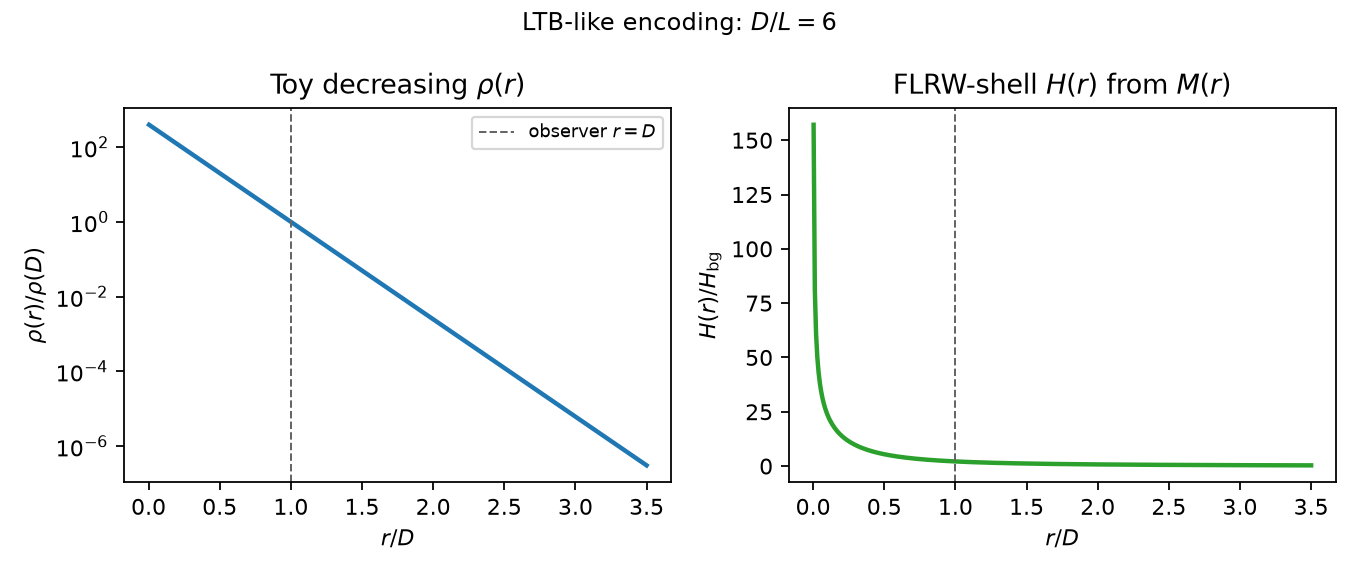
\includegraphics[width=\textwidth]{toy_density_H_profile.png}
\caption{Toy decreasing $\rho(r)$ from~\eqref{eq:rhotoy} and the corresponding
FLRW-shell $H(r)$ from~\eqref{eq:Hshell}, with observer at $r=D$ and $D/L=6$.
Centrally concentrated $M(r)$ produces higher $H$ near the CoE. This figure is
the density/curvature encoding step only---not yet an off-center sky map.}
\label{fig:profile}
\end{figure}

%----------------------------------------------------------------------
\section{Off-center observer geometry}
\label{sec:geom}

Place the CoE at the coordinate origin. The observer sits at areal / radial
coordinate distance $D$ from the CoE. A unit direction $\hat n$ on the
observer's sky makes an angle $\varphi$ with the CoE--observer axis:
$\varphi=0$ looks anti-center (away from the CoE), $\varphi=\pi$ looks toward
the CoE. In a planar toy,
\begin{equation}
  \hat n = (\cos\varphi,\sin\varphi),
  \qquad
  \mu\equiv\hat n\cdot\hat D=\cos\varphi.
\end{equation}
Sources at fixed observer-centric distance $s$ (survey-depth stand-in) have
CoE-radius
\begin{equation}
  r(\varphi)
  = \sqrt{D^2 + s^2 + 2 D s\cos\varphi}.
  \label{eq:rphi}
\end{equation}
The dimensionless ratios of interest match Chapter~1:
$d/D$ (here $s/D$ on the source circle; observer offset $/D = 1$ in units),
$D/L$, and mass contrast through $M(r)$.

\paragraph{Galactic longitude schematic.}
Comparing to Migkas $A(\ell)$ requires an overall sky-axis orientation: an
unknown angle between the CoE--observer axis and Galactic $\ell=0$. That
orientation is absorbed into a phase $\ell=\varphi+\ell_0$ scanned over
$[0,360^\circ)$. The phase is a geometric nuisance parameter, not a new force
law.

%----------------------------------------------------------------------
\section{Observables from null geodesics (pipeline)}
\label{sec:obs}

\subsection{What a finished calculation would do}

In a completed LTB treatment one integrates past-directed null geodesics from
the off-center observer, computes redshift $z(\hat n)$ and luminosity distance
$d_L(z,\hat n)$, and defines an effective direction-dependent Hubble rate from
the low-$z$ expansion
\begin{equation}
  d_L(z,\hat n)
  = \frac{cz}{H_{\mathrm{obs}}(\hat n)}
  + \mathcal{O}(z^2),
\end{equation}
or, more invariantly, uses the multipole decomposition of the general $d_L$
Hubble law~\citep{Heinesen2020}. CMB temperature along each ray follows from
the redshift of the last-scattering surface (or an equivalent photon
distribution), as in~\citet{Alnes2006,Kodama2010,Saito2010}.

\subsection{What this toy does}

The present shot replaces the geodesic $d_L$ map by the Chapter~1 sheet
convention applied to the FLRW-shell field:
\begin{equation}
  H_{\mathrm{obs}}(\varphi)
  \approx H\bigl(r(\varphi)\bigr),
  \qquad
  A(\varphi)
  = \frac{H_{\mathrm{obs}}(\varphi)}{\langle H_{\mathrm{obs}}\rangle}.
  \label{eq:toyA}
\end{equation}
This inherits the Newtonian scaffolding: it is honest about being a
local-$H$ / sheet-AF proxy, not Etherington reciprocity through curved null
congruences.

\paragraph{Amp$\times\sin$ and $2\ell$ as diagnostic residuals.}
As in Chapter~1, optional layers
\begin{align}
  A &\leftarrow A + \mathrm{Amp}\,\sin(\ell+\phi),
  \label{eq:ampsin}\\
  A &\leftarrow \bigl(1+\varepsilon\sin(2\ell+\psi)\bigr)A
  \label{eq:2ell}
\end{align}
may be fit after the geometric $A(\ell)$. They are \textbf{not} free parameters
of the LTB metric. They diagnose leftover phase and quadrupole structure
(axis misalignment, non-radial motion, strip geometry of Migkas bins, etc.).
The GR claim, such as it is, stops at the metric + off-center geometry +
observable map.

%----------------------------------------------------------------------
\section{Numerical toy calculation}
\label{sec:toy}

\subsection{Setup}

Parameters (dimensionless, then converted for CMB with $D\sim c/H_0$):
\begin{itemize}[leftmargin=*,itemsep=2pt]
\item Mass profile~\eqref{eq:Mtoy} with $D/L=6$.
\item Observer at $r=D$; sources on a circle with $s/D=0.5$ (Newtonian
  $d/D$ ballpark).
\item $H(r)$ from~\eqref{eq:Hshell}; $A$ from~\eqref{eq:toyA}.
\item Migkas comparison: digitised Fig.~6
  (\texttt{/workspace/cosmology/migkas/fig6\_digitized.csv}); affine $R^2$
  after best sky-axis phase.
\item Code: \texttt{scripts/toy\_offcenter\_ltb.py} with the project
  \texttt{.venv} Python.
\end{itemize}

\subsection{Migkas $A(\ell)$ result}

\begin{figure}[t]
\centering
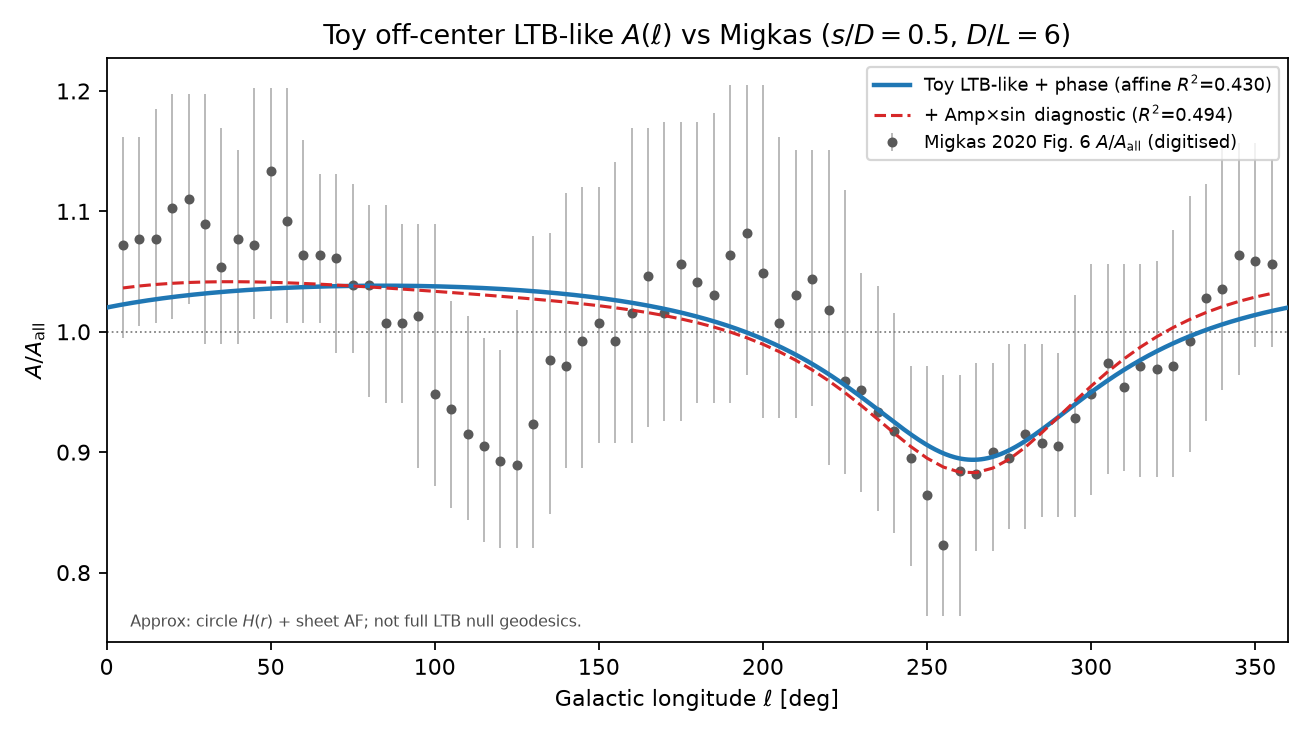
\includegraphics[width=0.92\textwidth]{A_vs_ell_toy_ltb.png}
\caption{Toy off-center LTB-like $A(\ell)$ (FLRW-shell $H(r)$ + sheet AF,
affine-matched after phase) versus digitised Migkas et~al.\ (2020) Fig.~6
$A/A_{\mathrm{all}}$. Geometry+phase affine $R^2\approx0.430$; adding a
diagnostic Amp$\times\sin$ layer reaches $R^2\approx0.494$. These $R^2$ values
are \emph{not} competitive with the Newtonian Chapter~1 ladder
($0.543\to0.746\to0.875$) and are not dressed up. Approximation: no full LTB
null geodesics.}
\label{fig:Aell}
\end{figure}

Reported numbers from the toy run:
\begin{center}
\begin{tabular}{@{}ll@{}}
\toprule
Quantity & Value \\
\midrule
$D/L$ & $6$ \\
$s/D$ (source circle) & $0.5$ \\
Best sky phase $\ell_0$ & $84^\circ$ \\
Affine $R^2$ (geometry + phase) & $\approx0.430$ \\
$R^2$ + Amp$\times\sin$ (diagnostic) & $\approx0.494$ \\
Best diagnostic Amp & $-0.15$ (grid edge; weak gain) \\
\bottomrule
\end{tabular}
\end{center}

The geometric angular shape is broadly dipolar in $\varphi$ after the sheet
map; Migkas $A(\ell)$ has additional structure that this FLRW-shell proxy does
not capture. Raising $R^2$ with Amp$\times\sin$ helps only modestly here---unlike
Chapter~1---which is itself information: the toy GR backbone is not yet carrying
the Newtonian template's full angular content.

%----------------------------------------------------------------------
\section{CMB kill-shot}
\label{sec:cmb}

Spherical symmetry plus an off-center observer generically produces a large CMB
temperature dipole. \citet{Alnes2006} showed that LTB void models fitted to SN
and the first CMB peak force the observer within $\sim15\,\mathrm{Mpc}$ of the
center once the COBE/WMAP-scale dipole is respected; analytic formulae
in~\citet{Saito2010,Kodama2010} recover the same ceiling
($\delta L\lesssim15$--$16\,\mathrm{Mpc}$). SNIa alone are much weaker on
centering~\citep{Alnes2006SN,Blomqvist2010}.

\paragraph{Linear toy estimate.}
At linear order in offset $d$,
\begin{equation}
  \Bigl|\frac{\delta T}{T}\Bigr|_{\mathrm{dipole}}
  \sim \bigl|\nabla\ln H\bigr|\,d,
  \label{eq:dip}
\end{equation}
with an Alnes-scaled reference curve
$(d/15\,\mathrm{Mpc})\times1.4\times10^{-3}$ matching their Model~I $a_{10}$
at $15\,\mathrm{Mpc}$. For the toy profile, evaluating $\nabla\ln H$ at
$r=D$ and taking $D\sim3000\,\mathrm{Mpc}$ (Hubble-length stand-in for a
beyond-horizon CoE) gives $|\nabla\ln H|\sim4.85\times10^{-4}\,\mathrm{Mpc}^{-1}$,
so the observed dipole $\sim1.2\times10^{-3}$ is reached already at
\begin{equation}
  d_{\max}\sim 2.5\,\mathrm{Mpc}
\end{equation}
for \emph{this} steep centrally concentrated profile---tighter than the void
$\sim15\,\mathrm{Mpc}$ class because the Hubble gradient is larger. At the
Newtonian target $d\sim0.5\,D\sim1500\,\mathrm{Mpc}$, the same estimate yields
$|\delta T/T|\sim0.7$, orders of magnitude above the data. The Alnes-scaled
curve at that offset is $\sim0.14$---still fatal.

\begin{figure}[t]
\centering
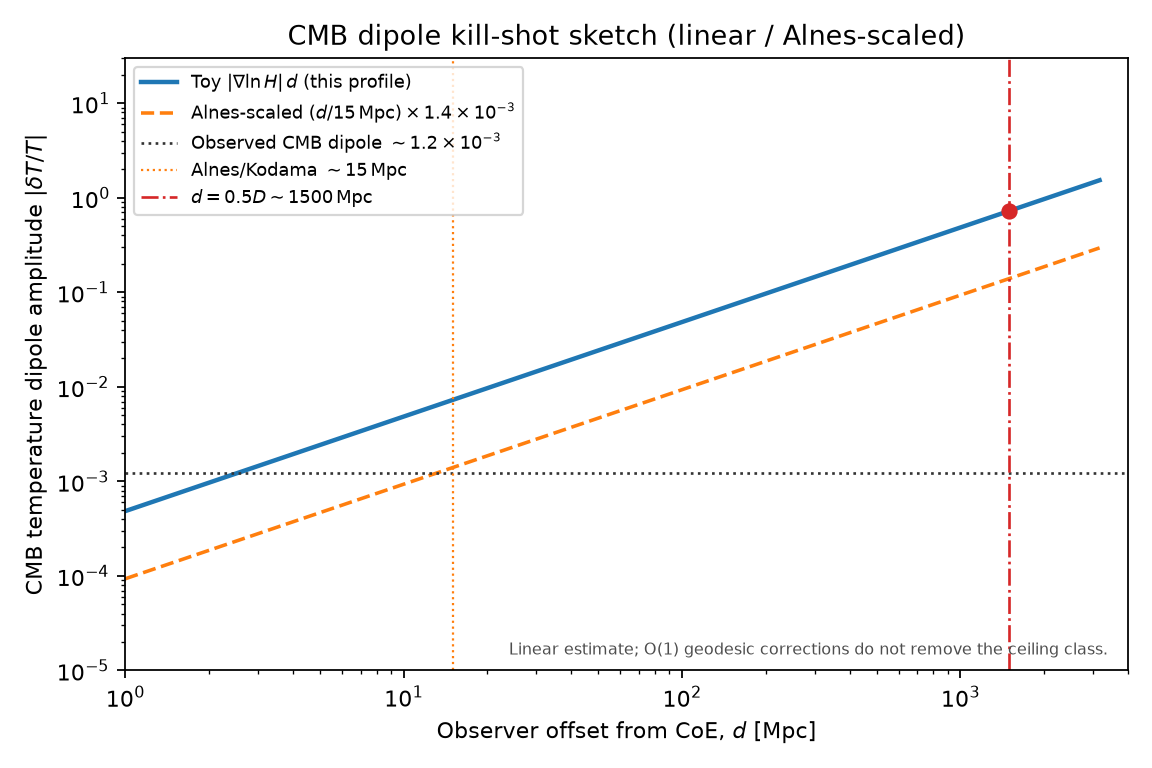
\includegraphics[width=0.85\textwidth]{cmb_dipole_vs_offset.png}
\caption{CMB dipole amplitude versus observer offset $d$. Solid: linear
$|\nabla\ln H|\,d$ for the toy profile with $D\sim3000\,\mathrm{Mpc}$. Dashed:
Alnes-scaled sketch
$(d/15\,\mathrm{Mpc})\times1.4\times10^{-3}$. Horizontal: observed CMB dipole
$\sim1.2\times10^{-3}$. Vertical: Alnes/Kodama $\sim15\,\mathrm{Mpc}$ and
Newtonian $d=0.5D$. Full geodesic LTB can change $O(1)$ factors; it does not
remove the ceiling class for a horizon-scale spherical offset.}
\label{fig:cmb}
\end{figure}

\paragraph{Why beyond-horizon CoE is in tension.}
If the CoE lies beyond the observable horizon and we sit at a substantial
fraction of the Hubble length from it, spherical symmetry makes our sky look
into a huge radial gradient of expansion and gravitational potential. The CMB
dipole is the leading symptom. Kinematic subtraction of the observed dipole
does not automatically cancel a \emph{geometric} dipole of comparable or larger
size without fine-tuned compensation~\citep{Alnes2006}.

\paragraph{What would be needed to survive.}
\begin{enumerate}[leftmargin=*,itemsep=2pt]
\item \textbf{Tiny offset:} $d\lesssim\mathcal{O}(10)\,\mathrm{Mpc}$ in
  spherical models---Copernican fine-tuning relative to a Gpc-scale structure,
  and incompatible with Newtonian $d/D\sim0.5$ if $D$ is cosmological.
\item \textbf{Break spherical symmetry} enough to suppress the monopole-gradient
  dipole while retaining a Migkas-like $A(\ell)$---no longer pure LTB; requires
  controlled anisotropy or screening, with Saadeh et~al.\ Bianchi limits in
  mind~\citep{Saadeh2016} (see Sec.~\ref{sec:roadmap}).
\item \textbf{Compensating peculiar velocity / ISW} tuned against the geometric
  dipole at the $10^{-3}$ level---possible in principle, not natural, and must
  not ruin other multipoles~\citep{Alnes2006}.
\item \textbf{Reinterpret the CMB dipole} as mostly cosmological rather than
  kinematic---a major claim against the standard reading; needs a full
  Boltzmann+geodesic calculation, not a sketch.
\end{enumerate}
None of these is demonstrated here. The honest verdict of this toy: the Migkas
angular program and a beyond-horizon spherical CoE are in direct conflict under
standard CMB dipole accounting.

%----------------------------------------------------------------------
\section{Roadmap}
\label{sec:roadmap}

\paragraph{Bertschinger (1983).}
Cosmological self-similar blast waves in Einstein--de~Sitter~\citep{Bertschinger1983}
are the closest classical dynamics cousin to the Sedov--Taylor language of
Chapter~1. A later upgrade should replace the static toy $M(r)$ with a
Bertschinger-like self-similar shell / blast profile inside an expanding
background, then recompute off-center null geodesics.

\paragraph{Smoller--Temple (1998, 2002).}
Shock-wave cosmologies matching FRW to TOV, including placement beyond one
Hubble length inside a black hole~\citep{SmollerTemple1998,SmollerTemple2002},
are the closest GR ontology cousins for a beyond-horizon CoE. They do not by
themselves solve the off-center CMB dipole; they upgrade the matching and
global causal structure once the local LTB sketch is under control.

\paragraph{Heinesen multipoles.}
Forecasts for $d_L(z,\hat n)$ should eventually be phrased in the
model-independent multipole Hubble law~\citep{Heinesen2020}, so that Migkas-like
directional $D_L$ constraints can be compared without committing to FLRW
background language.

\paragraph{What we are not doing: Bianchi.}
Globally homogeneous but anisotropic Bianchi models are tightly constrained by
Planck temperature and polarization~\citep{Saadeh2016}: anisotropic expansion
odds $\sim121{,}000:1$ against among that class. This program is
\textbf{inhomogeneous} (spherical CoE + off-center observer), not Bianchi.
Saadeh does not directly kill LTB/ST-off-center, but it forbids casually
rebranding the anisotropy as universe-wide shear. Any survival route that
breaks spherical symmetry must still respect those CMB limits.

%----------------------------------------------------------------------
\section{Conclusions}
\label{sec:concl}

\paragraph{What this shot achieved.}
\begin{itemize}[leftmargin=*,itemsep=2pt]
\item A self-contained GR-native note stating LTB + decreasing-$M(r)$ +
  off-center geometry + sheet-$A$ pipeline.
\item A reproducible toy with two required figures: $A(\ell)$ vs Migkas and
  CMB dipole vs $d$.
\item Real (not fabricated) Migkas comparison: affine $R^2\approx0.43$
  (geometry+phase); Amp$\times\sin$ diagnostic $\approx0.49$.
\item An explicit CMB kill-shot ledger aligned with Alnes/Kodama, showing
  horizon-scale offsets are untenable in spherical symmetry under standard
  dipole accounting.
\end{itemize}

\paragraph{What remains open.}
Full LTB (or LTB+$\Lambda$) null geodesics for $d_L$ and $\delta T/T$;
Bertschinger self-similar mass profiles; Smoller--Temple global matching;
any non-spherical mechanism that could reconcile Migkas-scale $A(\ell)$ with
CMB isotropy without Copernican fine-tuning. Until those exist, Chapter~2 is a
sketch: metric language for the Newtonian template, and a clear statement of
the CMB wall.

\bigskip
\noindent\textbf{Acknowledgments.}
Conversations and formative input from Wolfgang Rindler and Luke Ackerman are
gratefully acknowledged.

\bibliographystyle{plainnat}
\bibliography{refs}

\end{document}
